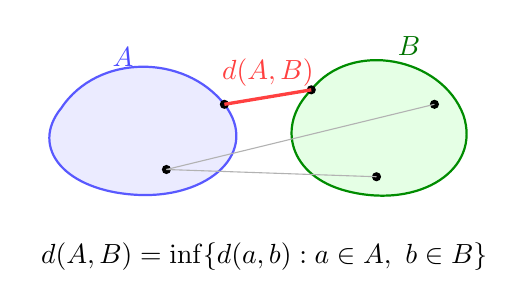
\begin{tikzpicture}[scale=0.92,>=stealth]
  \fill[blue!8]
    (-2.8,0.2) .. controls (-2.3,0.95) and (-1.1,0.95) .. (-0.55,0.25)
    .. controls (-0.05,-0.4) and (-0.75,-1.05) .. (-1.75,-1.0)
    .. controls (-2.75,-0.95) and (-3.25,-0.35) .. (-2.8,0.2);
  \draw[blue!65,thick]
    (-2.8,0.2) .. controls (-2.3,0.95) and (-1.1,0.95) .. (-0.55,0.25)
    .. controls (-0.05,-0.4) and (-0.75,-1.05) .. (-1.75,-1.0)
    .. controls (-2.75,-0.95) and (-3.25,-0.35) .. (-2.8,0.2);

  \fill[green!10]
    (0.65,0.45) .. controls (1.2,1.15) and (2.45,0.9) .. (2.75,0.1)
    .. controls (3.0,-0.65) and (2.15,-1.2) .. (1.15,-0.95)
    .. controls (0.35,-0.75) and (0.15,-0.05) .. (0.65,0.45);
  \draw[green!55!black,thick]
    (0.65,0.45) .. controls (1.2,1.15) and (2.45,0.9) .. (2.75,0.1)
    .. controls (3.0,-0.65) and (2.15,-1.2) .. (1.15,-0.95)
    .. controls (0.35,-0.75) and (0.15,-0.05) .. (0.65,0.45);

  \coordinate (a) at (-0.55,0.25);
  \coordinate (b) at (0.65,0.45);
  \coordinate (a2) at (-1.35,-0.65);
  \coordinate (b2) at (1.55,-0.75);
  \coordinate (b3) at (2.35,0.25);

  \foreach \p in {a,a2,b,b2,b3}
    \fill[black] (\p) circle (1.8pt);

  \draw[gray!60] (a2) -- (b2);
  \draw[gray!60] (a2) -- (b3);
  \draw[red!75,very thick] (a) -- (b)
    node[midway,above] {\(d(A,B)\)};

  \node[blue!70] at (-1.95,0.9) {\(A\)};
  \node[green!45!black] at (2.0,1.05) {\(B\)};
  \node[align=center] at (0,-1.85)
    {\(d(A,B)=\inf\{d(a,b):a\in A,\ b\in B\}\)};
\end{tikzpicture}
